% !TeX spellcheck = de_DE
\documentclass{beamer}

\usetheme{Madrid}
\usecolortheme{beaver}

% Navigation Symbols off
\beamertemplatenavigationsymbolsempty{}
%\usenavigationsymbolstemplate{}
\setbeamercolor*{item}{fg=red}
\setbeamercolor{itemize item}{fg=red} % all frames will have red bullets
% Watermark
\usebackgroundtemplate{%
	\rule{0pt}{\paperheight}%
	\hspace*{\paperwidth}%
	\makebox[0pt][r]{\includegraphics[width=60mm]{\resWatermark}}}

\usepackage[utf8]{inputenc}
\usepackage[german]{babel}
\usepackage[square,sort,comma,numbers]{natbib}
\usepackage{bibentry}
\usepackage{hyperref}
\usepackage{graphicx}
\usepackage{tikz}

% Logos
\newcommand{\resLogo}{../images/logo}
\newcommand{\resFBI}{../images/logo_fbi}
\newcommand{\resLogoSingle}{../images/logo_uhh}
\newcommand{\resWatermark}{../images/watermark}
% --- Commands ---
\renewcommand{\bibsection}{\subsubsection*{\bibname }}

% Custom commands
\newcommand{\gqq}[1]{\glqq#1\grqq} % encloses words in German quotes

\title{Ansätze und Verfahren der Datenmigration}
\subtitle{Datenmigration im Kontext des Reengineering}
\author[Schenkemeyer, Fechner]{\includegraphics[height=1cm]{\resLogo}\\Julian Schenkemeyer, Tobias Fechner\\ \texttt{\footnotesize\{5schenke,1fechner\}@informatik.uni-hamburg.de}}
\institute[UHH]{Universität Hamburg}
\date{\today}

% Section Heading
\AtBeginSection{\frame{
		\frametitle{\insertsection}
		\tableofcontents[currentsection]}
	}


% === DOCUMENT ===
\begin{document}
	
	% === TITLE ===
	\begin{frame}
		\maketitle
	\end{frame}
	
	\addtobeamertemplate{frametitle}{}{%
		\begin{tikzpicture}[remember picture, overlay]
		\node[anchor=north east,yshift=2pt, xshift=2pt] at (current page.north east) {%
			\includegraphics[height=.75cm]{\resFBI}\hspace{3pt}%
			\includegraphics[height=.75cm]{\resLogoSingle}%
		};
		\end{tikzpicture}
	}
	
	% === AGENDA ===
	
	\begin{frame}
		\frametitle{Agenda}
		\tableofcontents
	\end{frame}
	
	% ===========================================================================================================
	% ======= BEGIN CONTENT =====================================================================================
	% ===========================================================================================================
	
	\section{Datenmigration im Kontext des Reengineering}
	
	\begin{frame}
		\frametitle{Datenmigration - Definition}
		
		\textit{''Data migration is the selection, preparation, extraction, transformation and
		permanent movement of appropriate data that is of the right quality to the
		right place at the right time and the decommissioning of legacy data stores''} \cite{morris-2012}
	\end{frame}
	
	\begin{frame} %TODO Eventuell optional
		\frametitle{Riskien der Datenmigration \cite{morris-2012}}
		
		\begin{itemize}
			\item Unterschätzen der Datenmigration
			\item[]
			\item F"alschliche Technologiezentrierung
			\item[]
			\item Mangel an Spezialisten
%			\item[]
%			\item Gegenseitige Problemzuweisung
		\end{itemize}
	\end{frame}
	
	% ===========================================================================================================
	\section{Generelles Vorgehen}
	
	\begin{frame}
		\frametitle{Prozessmodell der Datenmigration}
				
		\centering
		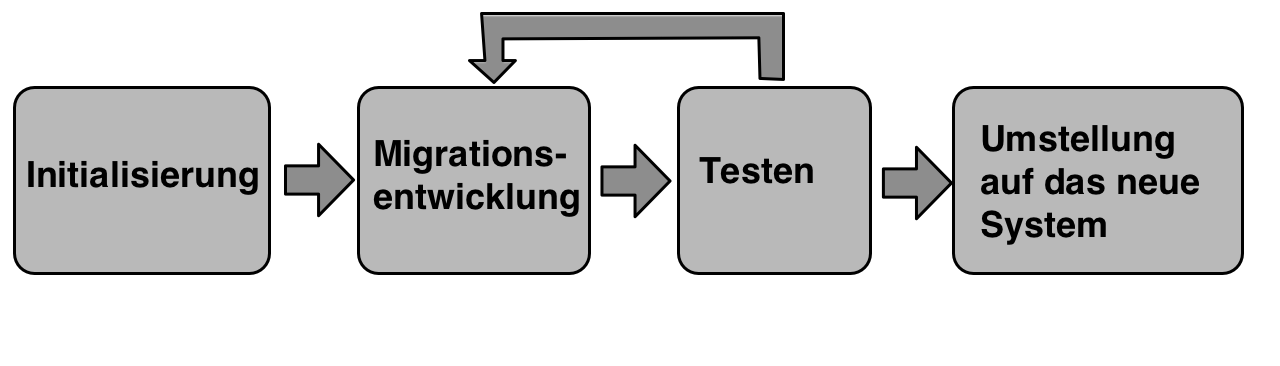
\includegraphics[width=\textwidth]{../images/prozessmodellt.png}
	\end{frame}
	
	\begin{frame}
		\frametitle{Abschnitt 1 - Initialisierung}
		
		\centering
		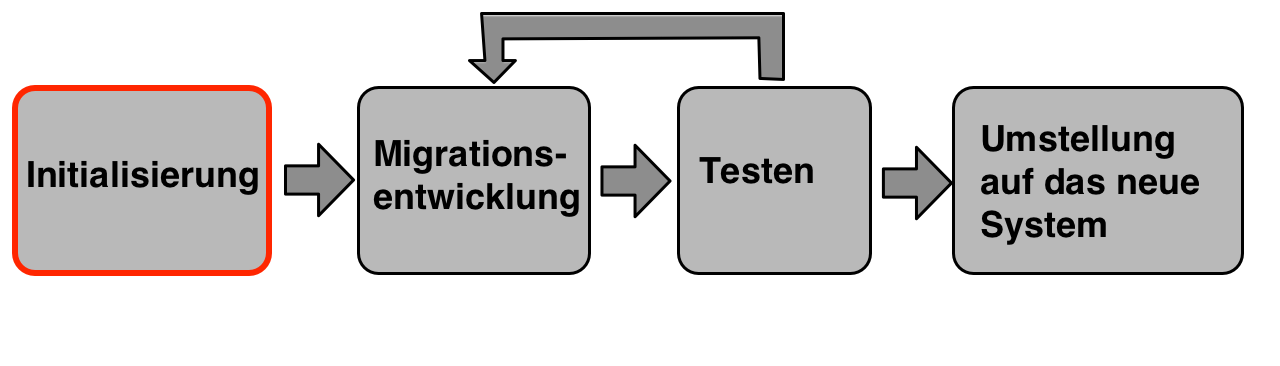
\includegraphics[width=\textwidth]{../images/prozessmodell1t.png}\\
	
		
		\begin{enumerate}
			\item \textbf{Initialisierung}
			\begin{itemize}
				\item Um was für ein Legacy-System handelt es sich?
				\item Welche Daten sollen auf das neue System übertragen werden?
				\item[]
				\item Entscheidung dar"uber, welche Vorgehensweise verwendet werden soll
				\item Initiale Aufwandseinschätzung
				\item Einrichten einer %TODO Satz fehlt noch
			\end{itemize}
		\end{enumerate}
	\end{frame}
	
	\begin{frame}
		\frametitle{Abschnitt 2 - Initialisierung}
		
		\centering
		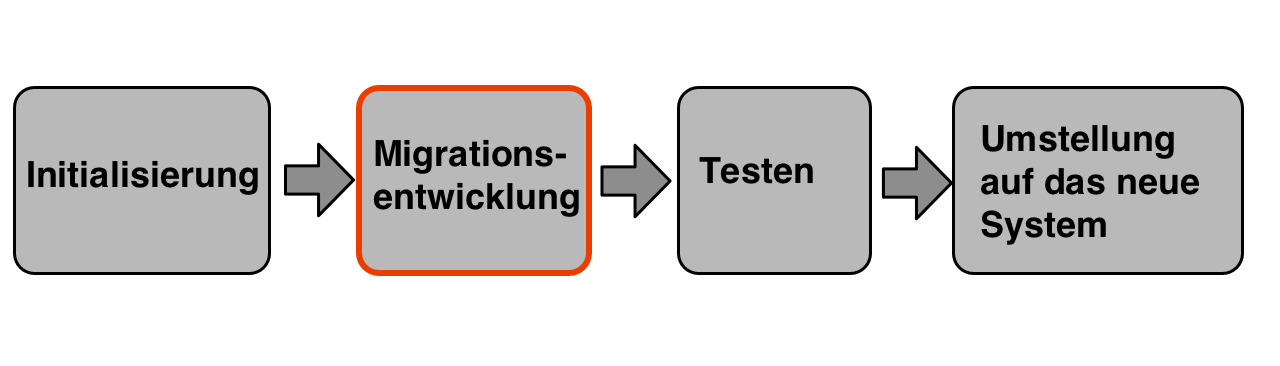
\includegraphics[width=\textwidth]{../images/prozessmodell2t.png}\\
		
		\begin{enumerate}
			\setcounter{enumi}{1}
			
			\item \textbf{Migrationsentwicklung}
			\begin{itemize}
				\item "Uberspielen eines Datenbackup auf die Migrationsplattform
				\item Vertiefende Analyse der Datenbest"ande des Legacy-Systems
				\item Entwicklung der Migrationsskripte und -werkzeuge
				\item Evtl. Durchf"uhrung von Data-Cleansing
			\end{itemize}
			
		\end{enumerate}
	\end{frame}
	
	\begin{frame}
		\frametitle{Abschnitt 3 - Testen}
		
		\centering
		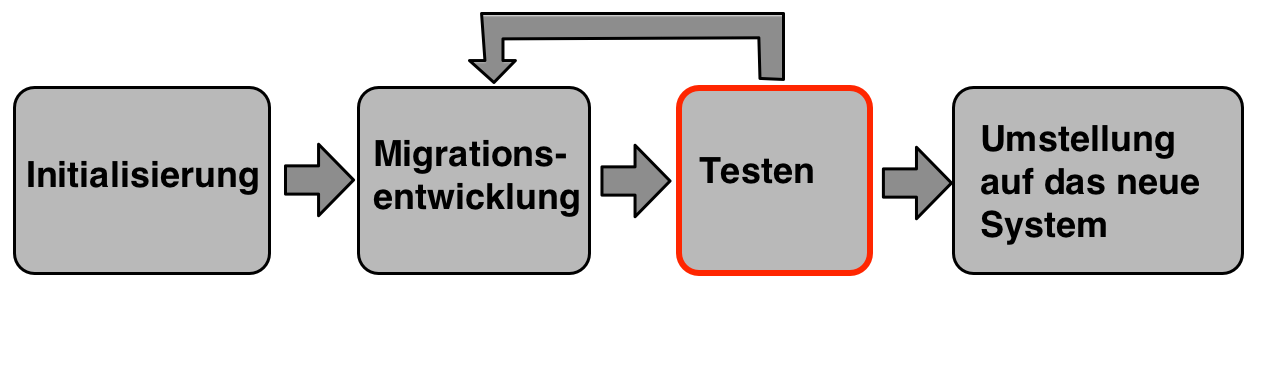
\includegraphics[width=\textwidth]{../images/prozessmodell3t.png}\\
		
		\begin{enumerate}
			\setcounter{enumi}{2}
			
			\item \textbf{Testen}
			\begin{itemize}
				\item "Uberpr"ufung von Funktionalit"at der Migrationsskripte
			\end{itemize}
			
		\end{enumerate}
	\end{frame}
	
	\begin{frame}
		\frametitle{Abschnitt 4 - Umstellung auf das neue System}
		
		\centering
		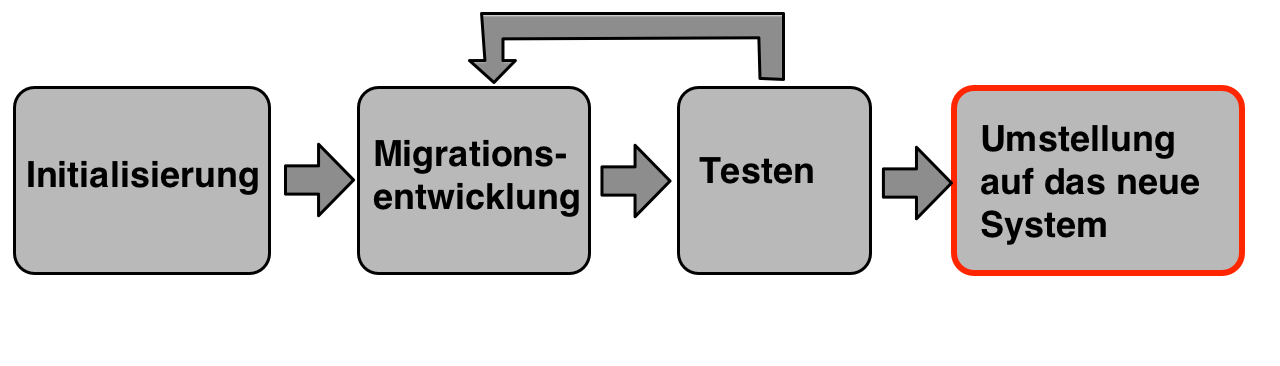
\includegraphics[width=\textwidth]{../images/prozessmodell4t.png}\\
		
		\begin{enumerate}
			\setcounter{enumi}{3}
						
			\item \textbf{Umstellung auf das neue System}
			\begin{itemize}
				\item Je nach gew"ahlter Vorgehensweise verl"auft dieser Abschnitt unterschiedlich
				\newline
				\item Erstellung eines Erfahrungsberichts
			\end{itemize}
			
		\end{enumerate}
	\end{frame}
	% ===========================================================================================================
	\section{Strategien zur Datenmigration}
	
	\begin{frame}
		\frametitle{Strategien der Datenmigration}
		
		\begin{itemize}
			\item Strategien mit unterschiedlichen Schwerpunkten
			\item[]
			\item Unterschiedliche Schwerpunkte erfordern unterschiedliches technisches und fachliches Wissen
			\item[]
			\item "Anderungen in Datenhaltung ziehen "Anderungen in nutzenden Anwendungen nach sich
			\item[]
			\item Ziel ist die Erhaltung von Daten
		\end{itemize}
	\end{frame}
	
	\subsection{Datenbankebene}
	
	\begin{frame}
		\frametitle{Datenbankebene}
		
		\begin{itemize}
			\item \textbf{Physisch}
				\begin{itemize}
					\item "Ubertrag von Daten
					\item H"aufig Portierung auf neues DBMS, keine fachliche Analyse
					\item Niedriger Aufwand, gut automatisierbar
				\end{itemize}
			\item[]
			\item \textbf{Konzeptuell}
				\begin{itemize}
					\item Neukonzeptionierung der Datenhaltung
					\item Fachliche Betrachtung
					\item Hoher Aufwand, schlecht automatisierbar
				\end{itemize}
		\end{itemize}
	\end{frame}	
	
	\begin{frame}
		\frametitle{Konzeptuelle Konvertierung}
		
		\centering
		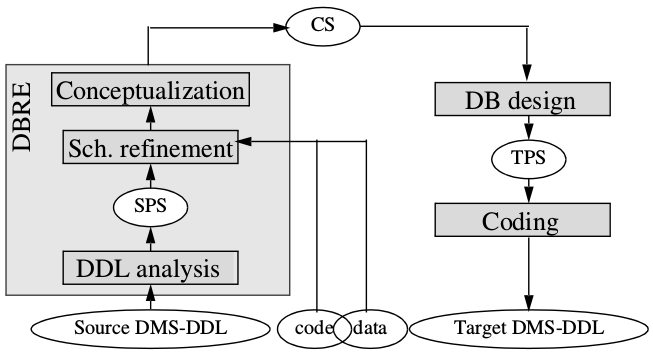
\includegraphics[height = 6cm]{../images/strategies_fig_02b.png}\\
		\tiny Quelle: \cite{henrard-2002}
	\end{frame}
	
	\subsection{Anwendungsebene}
	
	\begin{frame}
		\frametitle{Anwendungsebene}
		
		\begin{itemize}
			\item \textbf{Einsatz eines Wrappers} 
				\begin{itemize}
					\item Wrapper stellt Zugriff auf neue Datenquelle bereit
%					\item Anwendung benutzt Wrapper statt neue Datenquelle
%					\item Nutzung durch Wrapper f"ur Anwendung nur minimal ver"andert
					\item Niedriger Aufwand, erfordert wenig Kenntnisse der Anwendung
				\end{itemize}
			\item[]
			\item \textbf{Anpassung von Statements} 
				\begin{itemize}
					\item Aufrufe der Datenquelle werden angepasst
					\item Mittlerer Aufwand, erfordert mittlere Kenntnisse der Anwendung
				\end{itemize}
			\item[]
			\item \textbf{Anpassung der Zugriffslogik}
				\begin{itemize}
					\item Zugriffslogik wird angepasst
					\item Technische M"oglichkeiten der neuen Quellen k"onnen genutzt werden
					\item Hoher Aufwand, erfordert umfangreiche Kenntnisse der Anwendung
				\end{itemize}
		\end{itemize}
	\end{frame}
	
	\begin{frame}
		\frametitle{Vorgehen zur Einf"uhrung eines Wrappers}
		
		\centering
		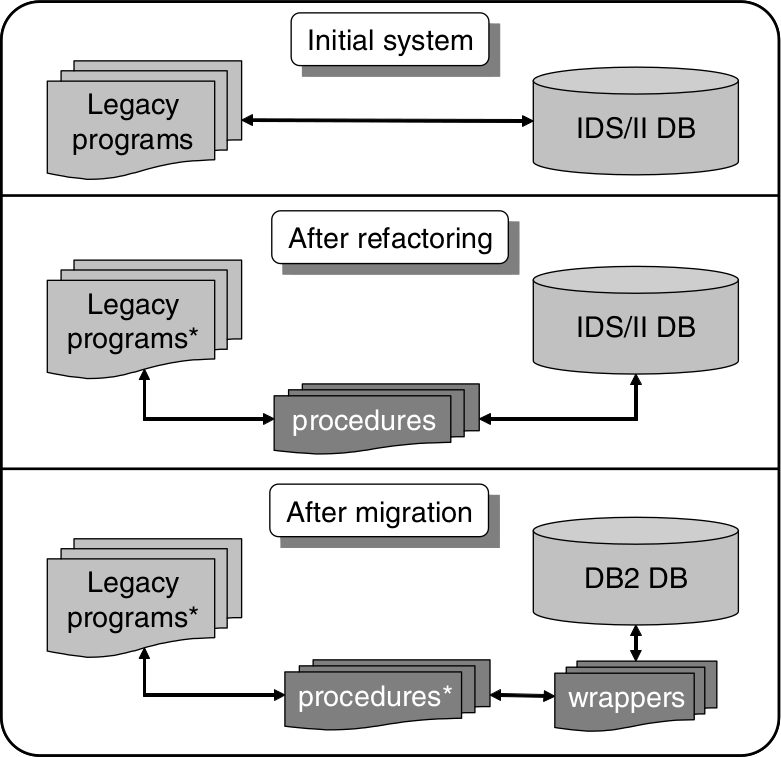
\includegraphics[height = 7cm]{../images/large_scale_fig_01.png} \\
		\tiny Quelle: \cite{henrard-2008}
	\end{frame}
	
	% ===========================================================================================================
	\section{Einf"uhrungsstrategien der Datenmigration}
	
	\subsection{}
	
	\begin{frame}
		\frametitle{Einf"uhrungsstrategien der Datenmigration}

		\begin{itemize}
			\item \textbf{Big-Bang-Ansatz}
				\begin{itemize}
					\item Datenmigration erfolgt auf einen Schlag
				\end{itemize}
			\item[]
			\item \textbf{Chicken-Little-Ansatz}
				\begin{itemize}
					\item Datenmigration erfolgt Modul für Modul
				\end{itemize}
			\item[]
			\item \textbf{Butterfly-Ansatz}
				\begin{itemize}
					\item Datenmigration erfolgt in Sch"uben
				\end{itemize}			
		\end{itemize}		
	\end{frame}
	
	\subsection{Butterfly-Ansatz}
	
	\begin{frame}
		\frametitle{Butterfly-Ansatz}
		
		\centering
		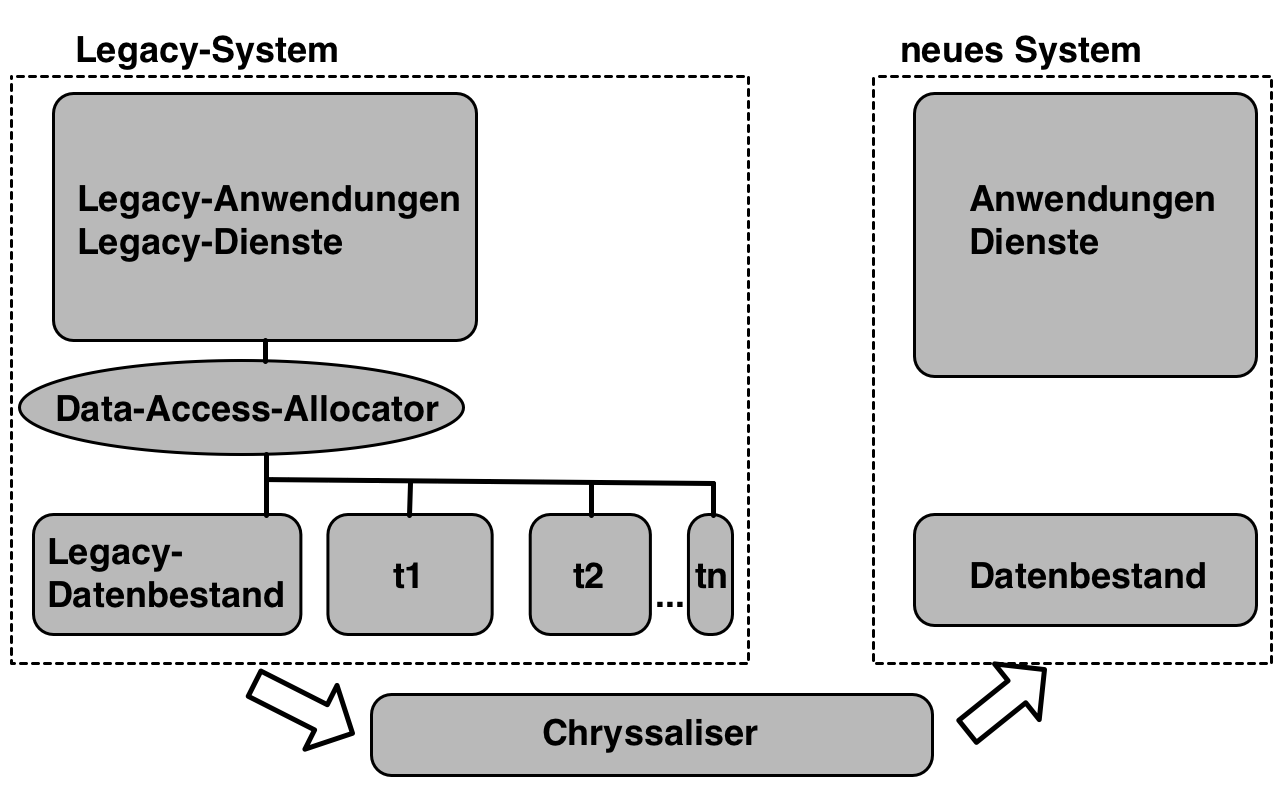
\includegraphics[width=0.95\textwidth]{../images/Butterfly.png} \\
		\tiny Quelle:  %TODO Hier noch die Quelle als Cite		
	\end{frame}
	
	\subsection{Vor- \& Nachteile der Ans"atze}
	\begin{frame}
		\frametitle{Einf"uhrungsstrategien der Datenmigration}
		
                \begin{footnotesize}
                \begin{table}[h]
                \centering
                \begin{tabular}{|p{1.5cm}|p{4.25cm}|p{4.25cm}|}
               
                \hline
                & \textbf{Vorteile} & \textbf{Nachteile} \\ 
		\hline
		\textbf{Big-Bang} & einfache Vorgehensweise & hohes Risiko \\
		\cline{3-3}
		& & Legacy-System während Migration nicht einsetzbar \\
		& & \\
		\hline
		
		\textbf{Chicken-Little} & Während Migration kann auf beiden Systemen gearbeitet werden & benötigt hohes fachliches Verständnis \\
		\cline{2-3}
		& Legacy-System kann Schrittweise ersetzt werden & Gateways können Performance verschlechtern \\
		\cline{3-3}
		& & kann sehr komplex werden \\
		& & \\
		\hline
		
		\textbf{Butterfly} & Während Migration kann auf dem Legacy-System weitergearbeitet werden & Data-Access-Allocator \& Chrysaliser müssen entwickelt werden \\
		\cline{2-3}
		& Zeitaufwand kann relativ sicher berechnet & Je nach Datenbestand hoher Hardwareaufwand \\
		& & \\
		\hline
		
		
		\end{tabular}
		\end{table}
		\end{footnotesize}
	
	\end{frame}
	
	
	% ===========================================================================================================
	\section{Fazit}
	
	\begin{frame}
		\frametitle{Fazit}
		
		Es gibt kein omnipotentes Verfahren zur Durchf"uhrung einer Datenmigration
		\begin{itemize}
			\item Welche Art von Unternehmen liegt vor?
			\item Welche Art von Legacy-System soll migriert werden?
			\item Welche Daten sollen migriert werden?
			\item Besteht schon ein ''neues System'' oder muss dieses erst entwickelt werden?
		\end{itemize}
	\end{frame}
	
	% ===========================================================================================================
	% ======= END CONTENT =======================================================================================
	% ===========================================================================================================
	
	% === QUELLEN ===
	%    \section{Quellen}
	
	\begin{frame}
		\frametitle{Quellen}
						
		\bibliographystyle{plaindin}
		\bibliography{../bib/mproj}
	\end{frame}
	
\end{document}
